% Дополнение к первой демонстрации (Демонстрация.pptx).
% Слайды 2--6 --- исходные схемы восприятия и вывода.
% Дальше --- архитектура памяти.
% Компиляция: pdflatex ah_hackathon.tex  (из этой папки, дважды)
% \newcommand{\DomainLine}{Цифровой двойник по корпусу учебных текстов}
\newcommand{\DomainLine}{предметная область --- вписать перед показом}

\documentclass[aspectratio=169,11pt]{beamer}

\usepackage[T2A]{fontenc}
\usepackage[utf8]{inputenc}
\usepackage[russian]{babel}
\usepackage{amsmath,amssymb}
\usepackage{graphicx}
\usepackage{tikz}
\usetikzlibrary{arrows.meta,positioning}

\usetheme{default}
\usecolortheme{default}
\setbeamertemplate{navigation symbols}{}
\setbeamertemplate{footline}{%
  \hfill\insertframenumber/\inserttotalframenumber\hspace{1em}\strut\par
}
\setbeamercolor{structure}{fg=black}
\setbeamercolor{frametitle}{fg=black}
\setbeamerfont{frametitle}{series=\bfseries,size=\large}

\tikzset{
  >={Stealth[length=2.2mm]},
  box/.style={
    draw, rectangle, align=center, inner sep=4pt, font=\scriptsize,
    minimum height=8mm, text width=28mm
  },
  layer/.style={
    draw, rectangle, align=center, inner sep=5pt, font=\small,
    minimum width=34mm, minimum height=16mm
  },
  src/.style={
    draw, rectangle, align=center, inner sep=3.2pt, font=\tiny,
    minimum height=20mm, text width=34mm
  },
  probe/.style={
    draw, rectangle, align=left, inner sep=3.2pt, font=\tiny,
    minimum height=20mm, text width=58mm
  },
  canon/.style={
    draw, rectangle, align=left, inner sep=3.2pt, font=\tiny,
    minimum height=20mm, text width=40mm
  },
}

\newcommand{\Lift}[1]{%
  {\scriptsize\textit{#1}}%
}

\title{От разбора предложения к канонической АГ-памяти}
\subtitle{Хакатон «Воспламенение 1.0»}
\author{команда AH Agent}
\date{}

\begin{document}

\begin{frame}
\titlepage
\vspace{-1.1em}
\begin{center}
{\small Алгоритмы сужают кандидатов, БЯМ закрывает неоднозначность, запись и вывод --- по правилам памяти.}\\[0.45em]
{\scriptsize \DomainLine}
\end{center}
\end{frame}

% ---- исходная демонстрация ------------------------------------------------
\begin{frame}{БЯМ только после сужения}
\begin{center}
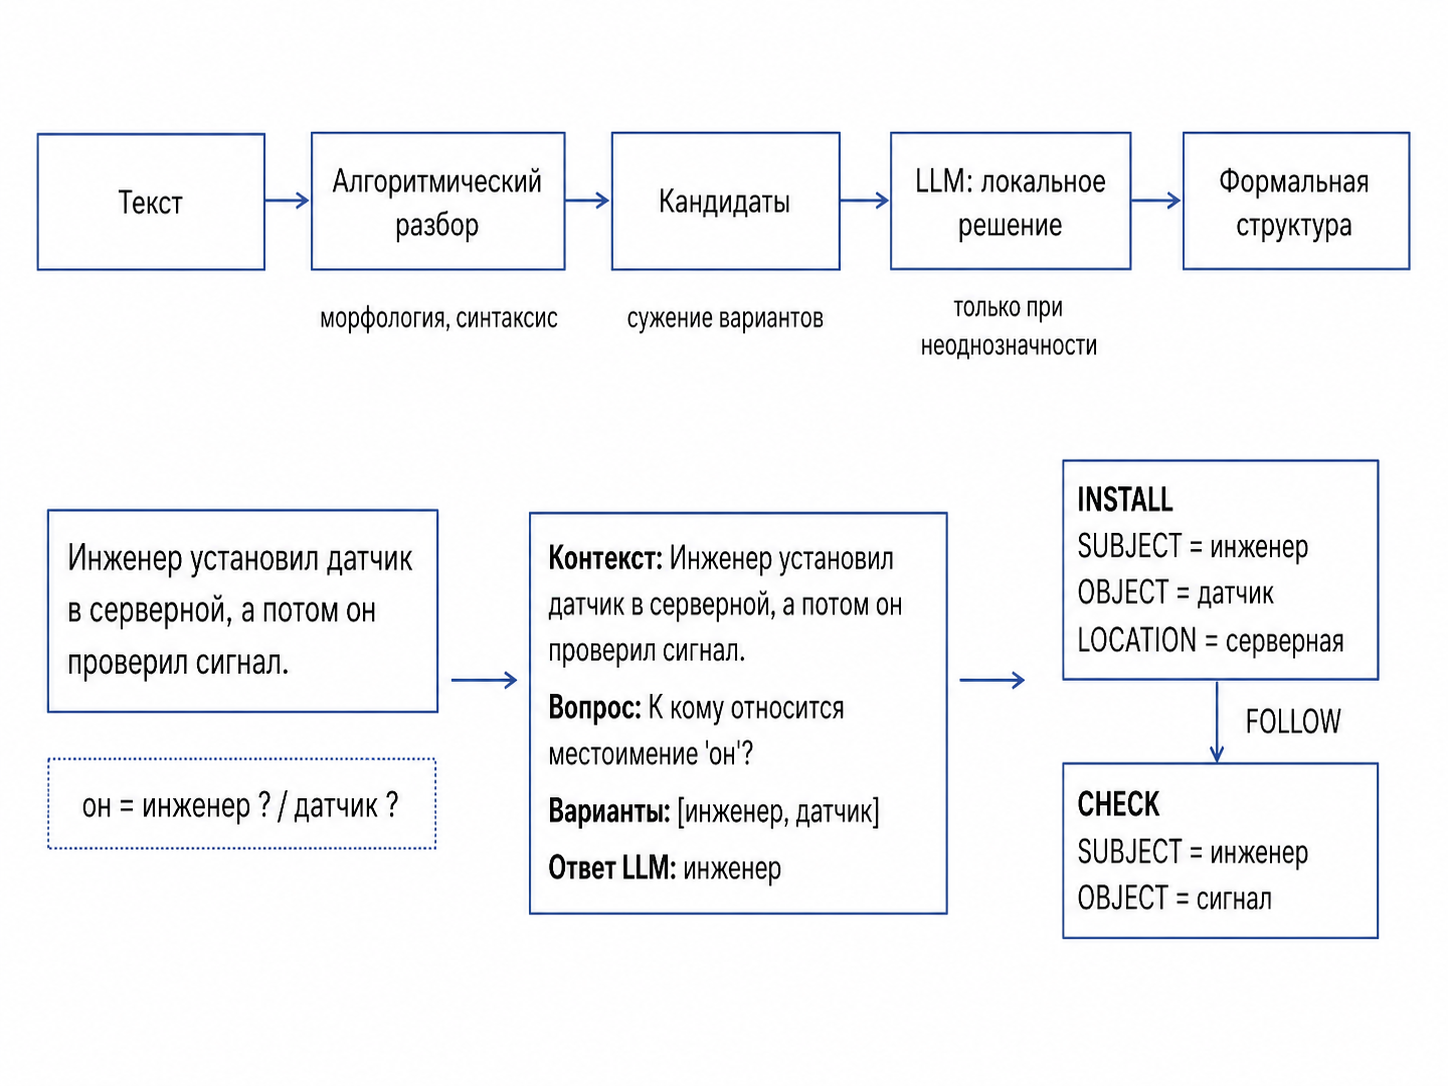
\includegraphics[width=0.98\textwidth,height=0.78\textheight,keepaspectratio]{figures/fig_perception.png}
\end{center}
\end{frame}

\begin{frame}{Морфология и границы групп}
\begin{center}
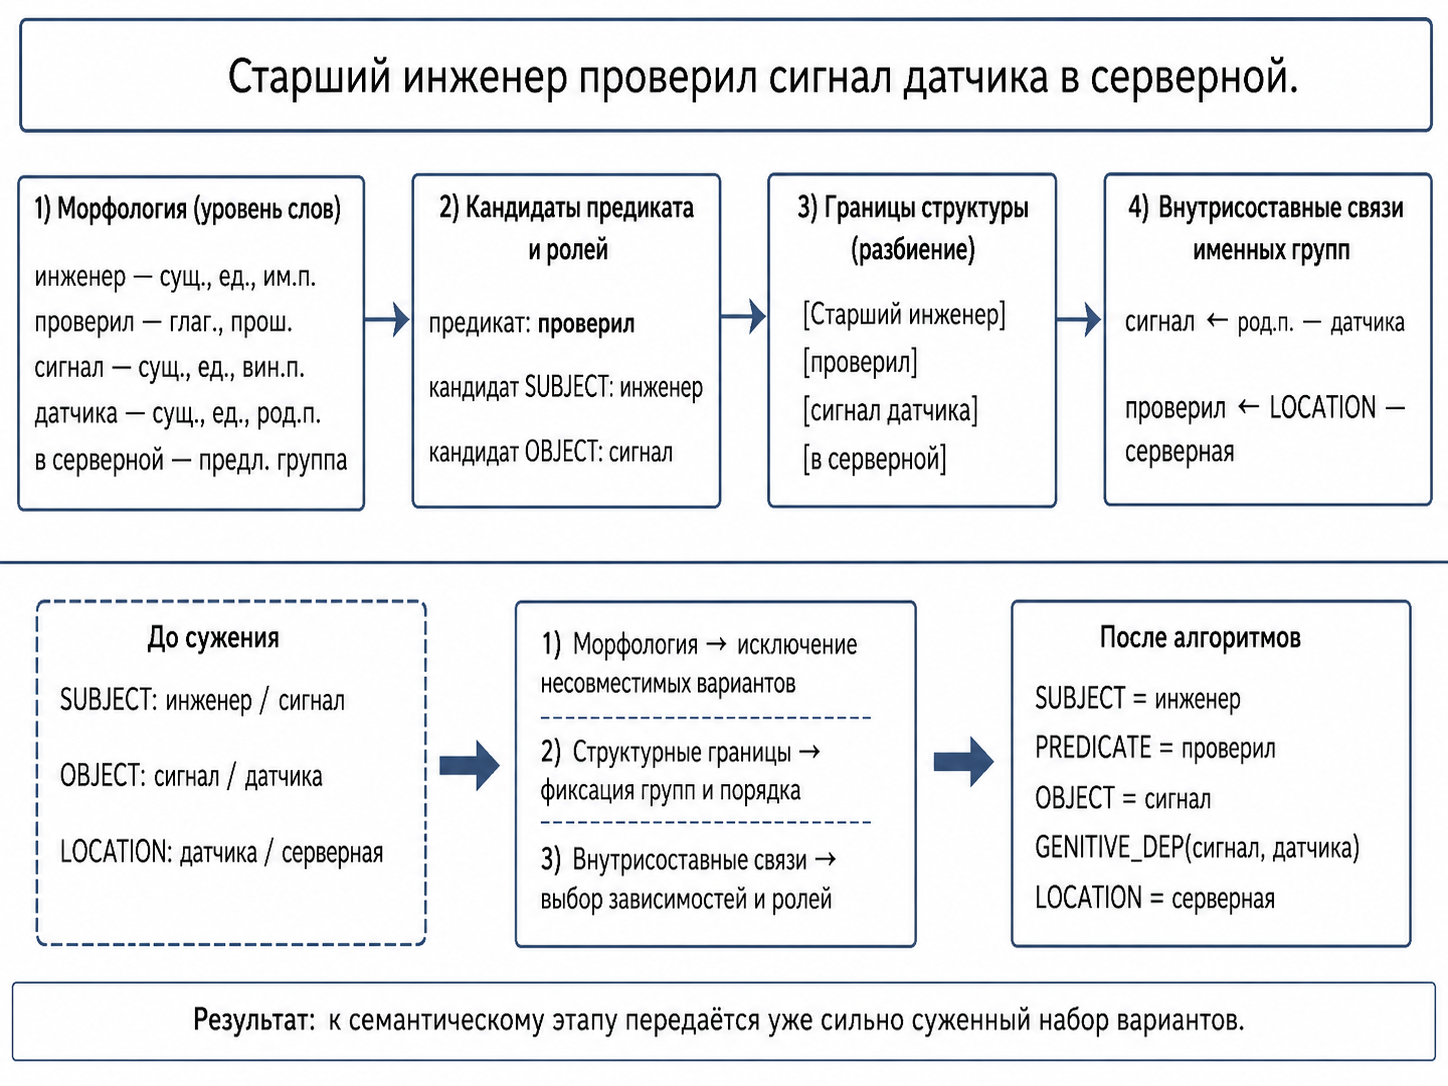
\includegraphics[width=0.98\textwidth,height=0.78\textheight,keepaspectratio]{figures/fig_morphology.png}
\end{center}
\end{frame}

\begin{frame}{Узкий вопрос к модели}
\begin{center}
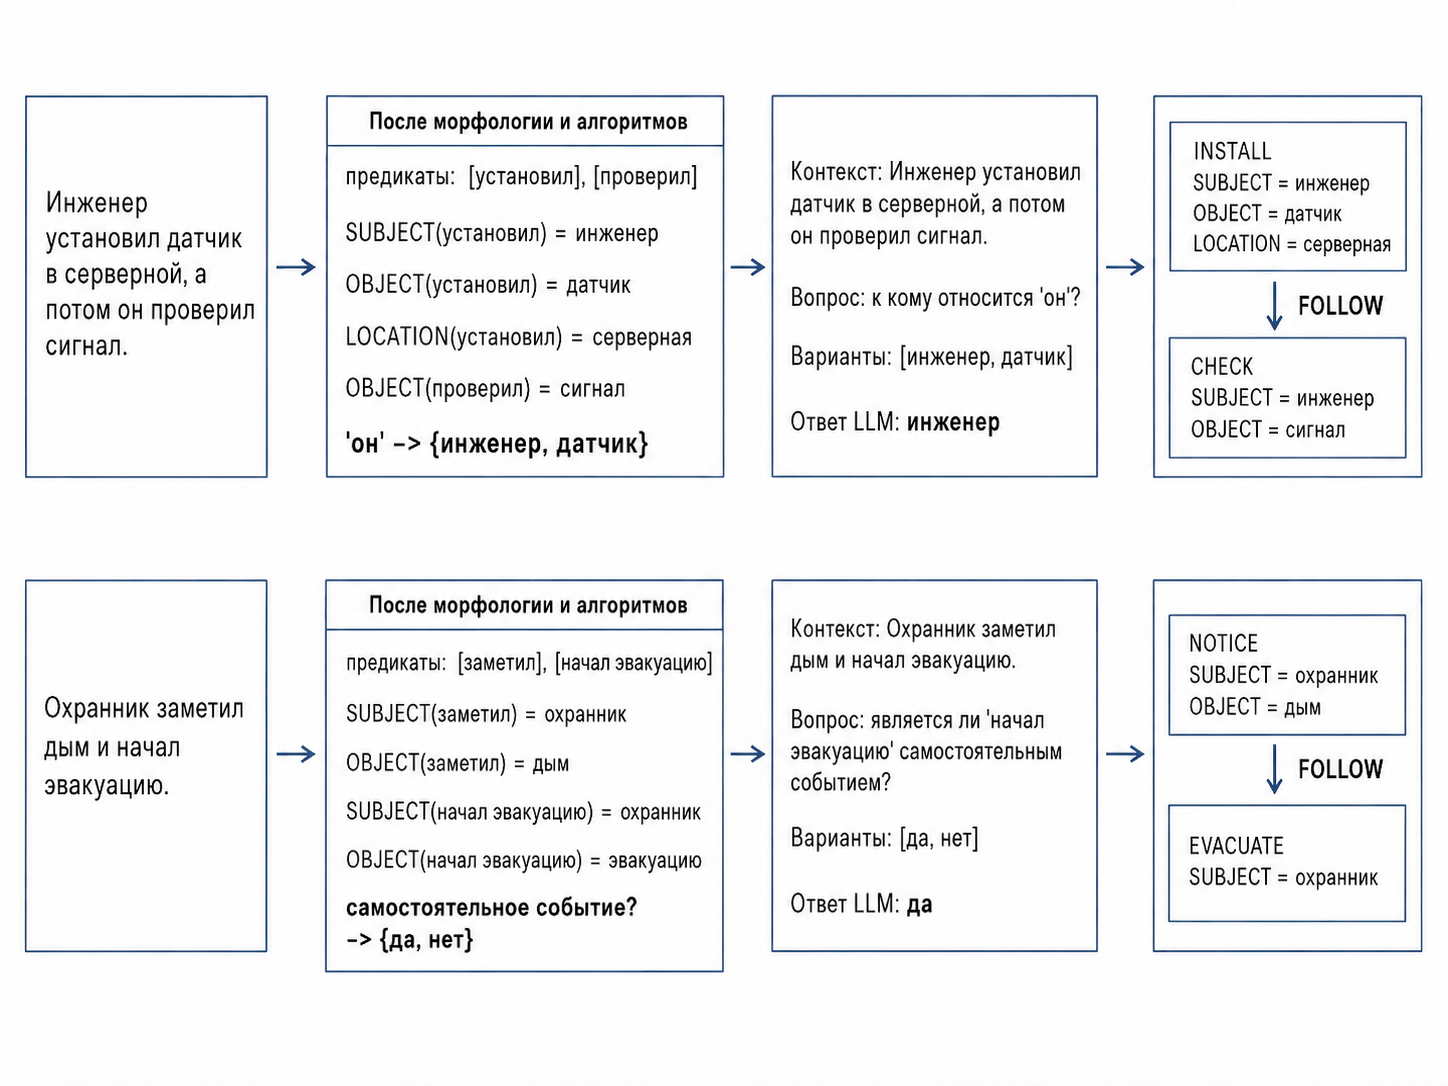
\includegraphics[width=0.98\textwidth,height=0.78\textheight,keepaspectratio]{figures/fig_llm_after.png}
\end{center}
\end{frame}

\begin{frame}{Неоднозначность фиксируется, не угадывается}
\begin{center}
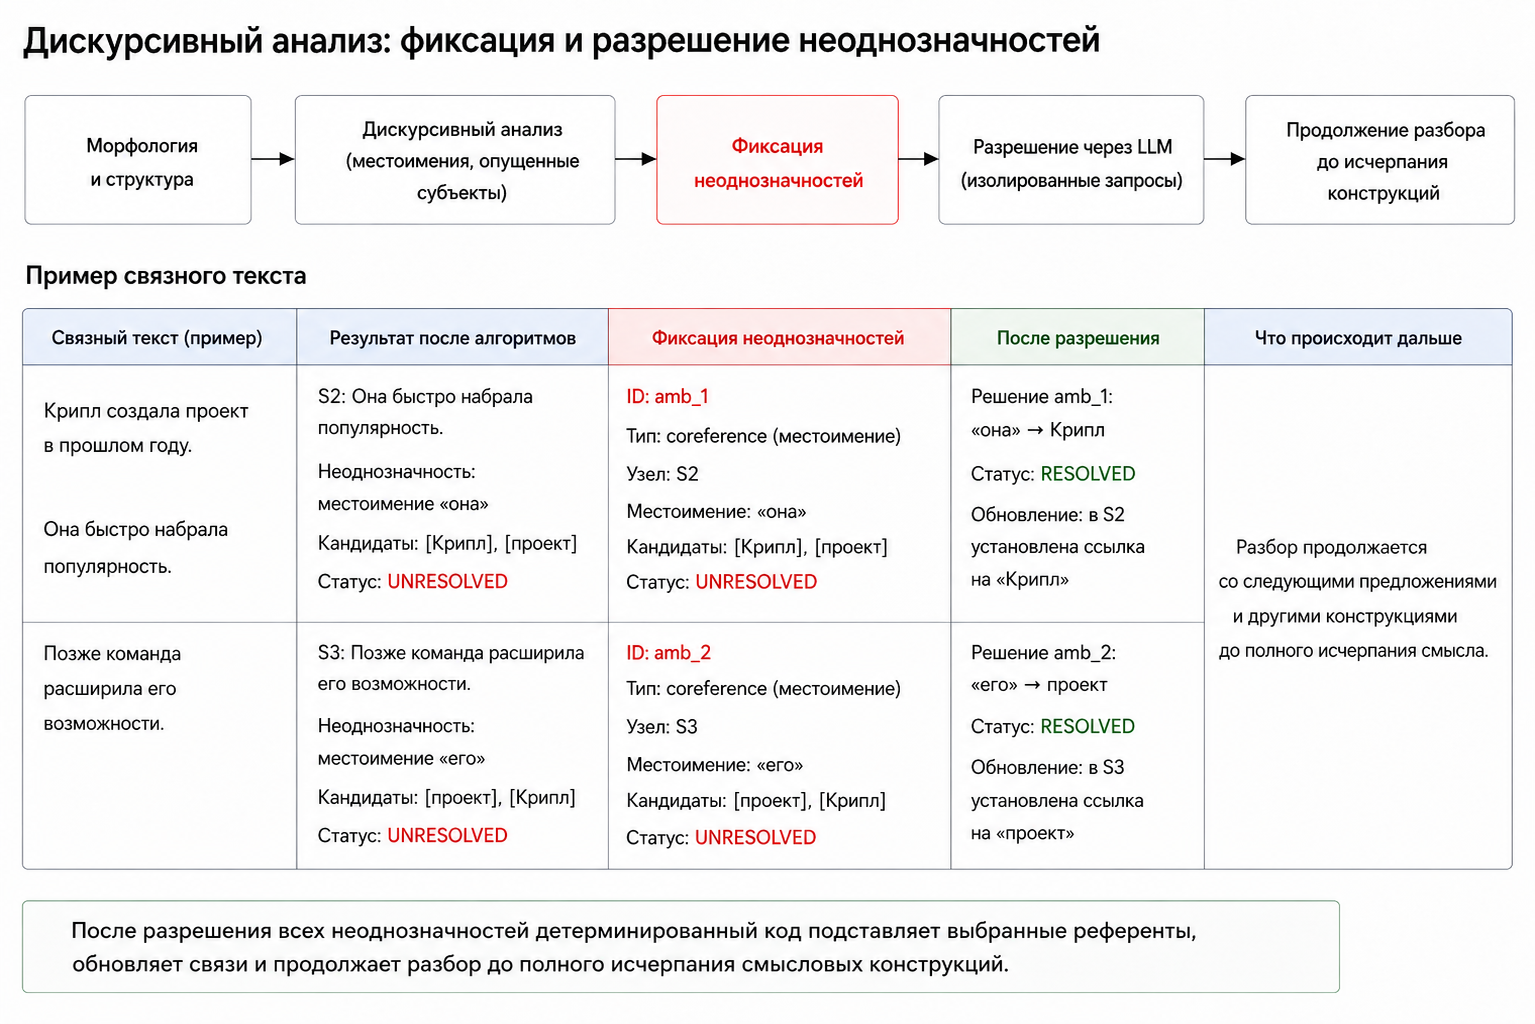
\includegraphics[width=0.98\textwidth,height=0.78\textheight,keepaspectratio]{figures/fig_discourse.png}
\end{center}
\end{frame}

\begin{frame}{Возбуждение находит, правила доказывают}
\begin{center}
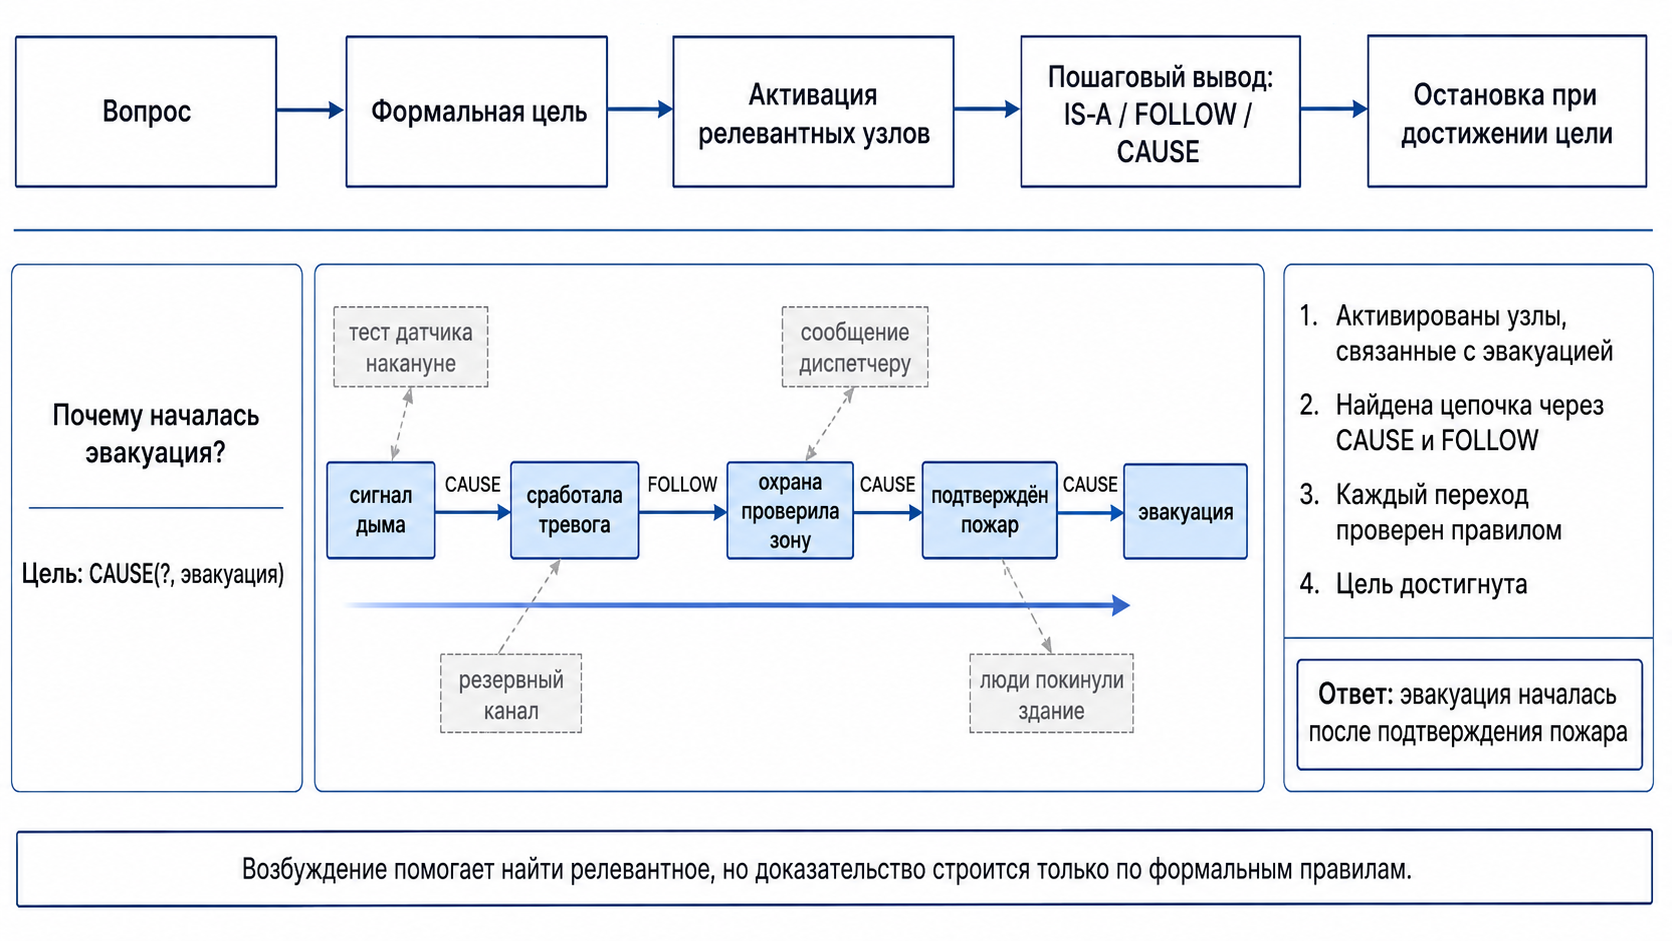
\includegraphics[width=0.98\textwidth,height=0.78\textheight,keepaspectratio]{figures/fig_proof.png}
\end{center}
\end{frame}

% ---- архитектура ----------------------------------------------------------
\begin{frame}{Каноническая память}
\begin{itemize}
  \item Память отдельно от runtime и от основной LLM.
  \item Atomic запись; равноправные кандидаты --- явная неоднозначность.
  \item Отложенная кореференция; Workspace; proof через такт ignition.
  \item Забывание сирот без вырезания живых цепочек.
\end{itemize}
\end{frame}

\begin{frame}{Три слоя: память, вычисление, генерация}
\vspace{-0.3em}
\begin{center}
\begin{tikzpicture}[node distance=8mm]
  \node[layer] (ah) {\textbf{Canonical AH}\\$S,C,P,H,L$\\что помнится};
  \node[layer, right=11mm of ah] (rt) {\textbf{Runtime}\\$x$, Workspace, proof\\DiscourseRef, BoundVar};
  \node[layer, right=11mm of rt] (llm) {\textbf{Main LLM}\\ответ\\не writer памяти};
  \draw[->, thick] (ah) -- (rt);
  \draw[->, thick] (rt) -- (llm);
\end{tikzpicture}
\end{center}
\vspace{0.55em}
\begin{itemize}
  \item Роли живут в $T/N$, не в промпте.
  \item Цепочка вывода адресуется UID, не текстом модели.
\end{itemize}
\end{frame}

\begin{frame}{Полный поток}
\vspace{-0.5em}
\begin{center}
\begin{tikzpicture}[node distance=2.2mm and 2.4mm, every node/.style={box, text width=20mm}]
  \node (txt) {текст};
  \node[right=of txt] (det) {детерм.\\разбор};
  \node[right=of det] (pr) {bounded\\probe};
  \node[right=of pr] (int) {atomic\\Integration};
  \node[below=8mm of int] (ah) {$AH$};
  \node[left=of ah] (ign) {Ignition};
  \node[left=of ign] (ws) {Workspace};
  \node[below=8mm of ws] (inf) {Recall / Proof};
  \node[right=of inf] (proj) {проекция};
  \node[right=of proj] (llm) {Main LLM};
  \node[right=of llm] (h) {ответ $\to H$};
  \draw[->] (txt) -- (det);
  \draw[->] (det) -- (pr);
  \draw[->] (pr) -- (int);
  \draw[->] (int) -- (ah);
  \draw[->] (ah) -- (ign);
  \draw[->] (ign) -- (ws);
  \draw[->] (ws) -- (inf);
  \draw[->] (inf) -- (proj);
  \draw[->] (proj) -- (llm);
  \draw[->] (llm) -- (h);
\end{tikzpicture}
\end{center}
\vspace{0.35em}
{\small Основная LLM \textbf{stateless}: нет history window. Прошлое входит в ответ только если возбуждено в Workspace.}
\end{frame}

\begin{frame}{Atomic Integration, fail-closed}
\begin{itemize}
  \item Запись --- только после полной проверки подграфа: $T$, актанты, identity, domain, дедуп.
  \item Полусозданные узлы в память не попадают.
  \item Равноправные кандидаты --- $k_{\mathrm{AMBIGUOUS}}$, не случайный выбор.
\end{itemize}
\vspace{0.5em}
\begin{center}
\begin{tikzpicture}[node distance=6mm, every node/.style={box, text width=32mm}]
  \node (a) {частичный граф\\и «модель допишет»};
  \node[right=12mm of a] (b) {commit целиком\\или ничего};
  \draw[->, thick] (a) -- (b);
\end{tikzpicture}
\end{center}
\Lift{опечатка, инверсия, эллипсис не порождают ложный факт.}
\end{frame}

\begin{frame}{Отложенная кореференция}
\begin{itemize}
  \item \texttt{DiscourseRef} --- staging, не узел AH. Якорь может появиться позже.
  \item Накопленные frames перепривязываются к $m$ до atomic commit.
  \item «Кто-то вошёл. Он сел.» $\to$ $\exists\,x\colon \mathrm{ENTER}(x)\land\mathrm{SIT}(x)$, без фиктивного $m_{\mathrm{UNKNOWN}}$.
\end{itemize}
\Lift{нет ложных сущностей и оборванных ролей на всём корпусе.}
\end{frame}

\begin{frame}{$T/N$ для предикатов, $L$ только структурные}
\begin{itemize}
  \item Новый глагол расширяет $T/N$, не плодит $L.\mathrm{ID}$.
  \item $L$ --- $IS\text{-}A$, $FOLLOW$, $CAUSE$ (то, что умеет reasoner).
  \item Слова «если / или» не включают $\mathrm{IMPLIES}$ / $\mathrm{OR}$.
\end{itemize}
\vspace{0.45em}
\begin{center}
\begin{tikzpicture}[node distance=6mm, every node/.style={box, text width=32mm}]
  \node (a) {keyword $\to$ ребро\\в графе};
  \node[right=12mm of a] (b) {структура предложения\\$\to$ $T/N$ или $g$};
  \draw[->, thick] (a) -- (b);
\end{tikzpicture}
\end{center}
\Lift{причинные и таксономические цепи короткие и проверяемые.}
\end{frame}

\begin{frame}{Формализация: какой тип --- $T$, $L$ или $g$}
\vspace{-0.45em}
\begin{center}
\begin{tikzpicture}[node distance=3.2mm, every node/.style={box, text width=26mm, minimum height=7mm, font=\tiny}]
  \node (a) {клаузы, NP,\\актанты};
  \node[right=of a] (b) {кандидаты\\типа};
  \node[right=of b] (c) {probe:\\один enum};
  \node[right=of c] (d) {$T$ / $L$ / $g$\\собирает Python};
  \draw[->] (a) -- (b);
  \draw[->] (b) -- (c);
  \draw[->] (c) -- (d);
\end{tikzpicture}
\end{center}
\vspace{0.15em}
\begin{center}
\begin{tikzpicture}[node distance=3.6mm]
  \node[src] (t1) {\textbf{текст}\\[0.2em]
    Инженер установил\\датчик в серверной.};
  \node[probe, right=of t1] (q1) {\textbf{вопрос к БЯМ}\\[0.15em]
    TARGET: «установил»\\
    English base-form predicate?\\
    ответ: \texttt{install}};
  \node[canon, right=of q1] (r1) {\textbf{тип $T/N$}\\[0.15em]
    $T_{\mathrm{INSTALL}}$\\
    $N(\mathrm{SUBJECT}{=}\mathrm{инженер}$,\\
    $\mathrm{OBJECT}{=}\mathrm{датчик})$};
  \draw[->] (t1) -- (q1);
  \draw[->] (q1) -- (r1);

  \node[src, below=4.2mm of t1] (t2) {\textbf{текст}\\[0.2em]
    Иван --- человек.};
  \node[probe, right=of t2] (q2) {\textbf{вопрос к БЯМ}\\[0.15em]
    Это $\mathrm{IS\text{-}A}$ listed referent?\\
    \texttt{R1}: Иван $\mathrm{IS\text{-}A}$ человек\\
    \texttt{NONE}: обычный предикат\\
    ответ: \texttt{R1}};
  \node[canon, right=of q2] (r2) {\textbf{тип $L$}\\[0.15em]
    $L{:}\ \mathrm{Иван}\xrightarrow{\mathrm{IS\text{-}A}}\mathrm{человек}$\\
    не новый $g.\mathrm{ID}$,\\
    не keyword «являться»};
  \draw[->] (t2) -- (q2);
  \draw[->] (q2) -- (r2);
\end{tikzpicture}
\end{center}
\Lift{модель называет тип из списка; UID и шаблон пишет Integration.}
\end{frame}

\begin{frame}{Формализация: квантор и импликация}
\vspace{-0.35em}
\begin{center}
\begin{tikzpicture}[node distance=3.6mm]
  \node[src] (t1) {\textbf{текст}\\[0.2em]
    Все люди смертны.};
  \node[probe, right=of t1] (q1) {\textbf{вопрос: TARGET «все люди»}\\[0.12em]
    \texttt{NONE} --- конкретный референт\\
    \texttt{EXISTS} / \texttt{NOT\_EXISTS}\\
    \texttt{FORALL} / \texttt{NOT\_FORALL}\\
    ответ: \texttt{FORALL}};
  \node[canon, right=of q1] (r1) {\textbf{тип $g$}\\[0.15em]
    $g_{\mathrm{FORALL}}(\$0,$\\
    $g_{\mathrm{IMPLIES}}($\\
    $\mathrm{HUMAN}(\$0),$\\
    $\mathrm{MORTAL}(\$0)))$};
  \draw[->] (t1) -- (q1);
  \draw[->] (q1) -- (r1);

  \node[src, below=4.2mm of t1] (t2) {\textbf{текст}\\[0.2em]
    Если датчик сработал,\\началась эвакуация.};
  \node[probe, right=of t2] (q2) {\textbf{вопрос: направление}\\[0.12em]
    \texttt{SUBORDINATE\_TO\_MATRIX}\\
    \texttt{MATRIX\_TO\_SUBORDINATE}\\
    \texttt{UNCLEAR}\\
    ответ: \texttt{SUBORDINATE\_TO\_MATRIX}};
  \node[canon, right=of q2] (r2) {\textbf{тип $g$}\\[0.15em]
    $g_{\mathrm{IMPLIES}}($\\
    $\mathrm{TRIGGER}(\mathrm{датчик}),$\\
    $\mathrm{EVACUATE})$\\
    «если» само $\neq$ $\mathrm{IMPLIES}$};
  \draw[->] (t2) -- (q2);
  \draw[->] (q2) -- (r2);
\end{tikzpicture}
\end{center}
\vspace{0.2em}
{\scriptsize
«Не все сотрудники пришли» $\to$ $\mathrm{NOT}(\mathrm{FORALL}\ldots\mathrm{CAME})$.
«Все сотрудники не пришли» $\to$ $\mathrm{FORALL}(\ldots\mathrm{NOT}(\mathrm{CAME}))$.
\texttt{AMBIGUOUS} / \texttt{UNCLEAR} $\to$ не запись.}
\end{frame}

\begin{frame}{Lexical Recovery до семантики}
\begin{itemize}
  \item Опечатка --- отдельный слой: словарь / автомат / морфология / рамка.
  \item Чат-БЯМ слово не «исправляет».
  \item Сырая форма --- provenance; в identity --- только уверенное исправление.
  \item Неоднозначное исправление --- fail-closed.
\end{itemize}
\Lift{шум не разваливает SUBJECT/OBJECT.}
\end{frame}

\begin{frame}{Workspace вместо окна чата}
\[
\mathrm{Workspace}_t = \{\, e \mid x_e > t \,\}
\]
\begin{itemize}
  \item Не отдельная память и не top-$N$ сниппетов.
  \item $\mathrm{activation} \neq \mathrm{truth} \neq \mathrm{proof}$.
  \item Вход LLM: запрос + проекция Workspace + результат proof.
\end{itemize}
\Lift{галлюцинация без UID в графе не проходит как знание.}
\end{frame}

\begin{frame}{Proof через такт ignition}
\begin{itemize}
  \item Recall: что стало релевантным. Inference: что следует по правилам.
  \item Шаг proof: focus $\to$ tick $\to$ сдвиг Workspace $\to$ следующий шаг.
  \item Обратное расстояние по графу --- эвристика кандидатов, не доказательство.
\end{itemize}
\vspace{0.35em}
\begin{center}
\begin{tikzpicture}[node distance=5mm, every node/.style={box, text width=26mm}]
  \node (a) {BFS, потом\\нарисовать след};
  \node[right=10mm of a] (b) {правило $\to$ tick\\$\to$ UID в трассе};
  \draw[->, thick] (a) -- (b);
\end{tikzpicture}
\end{center}
\Lift{пустая трасса $\neq$ вывод; цепочка совпадает с тем, что возбудилось.}
\end{frame}

\begin{frame}{Жизнь элемента и сборка мусора}
\begin{itemize}
  \item \texttt{initial\_lifetime} --- иммунитет, не приговор к удалению.
  \item Пульс $\nu$ и пол затухания \textbf{не} продлевают TTL.
  \item Спасает только $x>t$ или настоящее возбуждение. Живой S-якорь не вычищается возрастом.
\end{itemize}
\vspace{0.4em}
\begin{center}
\begin{tikzpicture}[node distance=6mm, every node/.style={box, text width=32mm}]
  \node (a) {пейсмекер = жизнь\\сироты копятся};
  \node[right=12mm of a] (b) {сирота уходит,\\связное остаётся};
  \draw[->, thick] (a) -- (b);
\end{tikzpicture}
\end{center}
\Lift{граф операбелен: нет фиктивных гиперузлов и вырезания живых цепочек.}
\end{frame}

\begin{frame}{RAG снаружи, шаблоны $T$ внутри}
\begin{itemize}
  \item Сырой текст --- provenance, не retrieval-память.
  \item Векторный поиск --- отдельный пакет, \textbf{не пишет} в память.
  \item Жёсткие шаблоны $T$ и обязательные SUBJECT/OBJECT --- один парсер для любой модели.
\end{itemize}
\Lift{слоты задаёт каркас, не промпт.}
\end{frame}

\begin{frame}{Регламент защиты}
\begin{enumerate}
  \item Новый ЕЯ-факт $\to$ automatic commit и UID.
  \item Вопрос $\ge 3$ шага по $FOLLOW$ / $IS\text{-}A$ / $CAUSE$ и трасса тактов.
  \item Пять гиперпараметров; меняем один --- видно затухание, порог Workspace или жизнь сирот.
\end{enumerate}
\vspace{0.7em}
\begin{block}{На экране}
Канонический узел $\to$ возбуждение $\to$ Workspace $\to$ proof с UID.
\end{block}
\end{frame}

\end{document}
